\documentclass[10pt]{article}

\usepackage[margin=0.75in]{geometry}
\usepackage{amsmath,amsthm,amssymb}
\usepackage{xcolor}
\usepackage{cancel}
\usepackage{graphicx}
\usepackage{changepage}
\usepackage{circuitikz}
\usepackage{pgfplots}
\usepackage{physics}
\usepackage{hyperref}
\usepackage{siunitx}
\usepackage[breakable]{tcolorbox}
\usepackage[inline]{enumitem}

\theoremstyle{definition}
\newtheorem{problem}{Problem}
\newtheorem{soln}{Solution}

\pgfplotsset{compat=newest}
\usetikzlibrary{arrows, angles, calc, quotes}

\definecolor{incolor}{HTML}{303F9F}
\definecolor{outcolor}{HTML}{D84315}
\definecolor{cellborder}{HTML}{CFCFCF}
\definecolor{cellbackground}{HTML}{F7F7F7}
\newcommand{\eq}{=}
\usetikzlibrary{positioning, fit, calc}
\pgfdeclarelayer{background}  
\pgfsetlayers{background,main}
\DeclareSIUnit[number-unit-product = {\,}]\calorie{cal}
\DeclareSIUnit[number-unit-product = {\,}]\atmosphere{atm}
\AtBeginDocument{\RenewCommandCopy\qty\SI}

\makeatletter
\newcommand{\boxspacing}{\kern\kvtcb@left@rule\kern\kvtcb@boxsep}
\makeatother
\newcommand{\prompt}[4]{
    \ttfamily\llap{{\color{#2}[#3]:\hspace{3pt}#4}}\vspace{-\baselineskip}
}

\newcommand{\thevenin}[2]{
  \begin{center}
    \begin{circuitikz} \draw
      (0,0) -- (2,0) to[battery1, l_=$V_{Th}\eq#1$] (2,2) 
      to[resistor, l_=$R_{Th}\eq#2$] (0,2)
      ;
      \draw [o-] (-.07,2.079);
      \draw [o-] (-.07,0.079);
    \end{circuitikz}
  \end{center}
}

\newcommand{\norton}[2]{
  \begin{center}
    \begin{circuitikz} \draw
      (0,0) -- (3,0) to[american current source, l_=$I_{N}\eq#1$] (3,2) -- (0,2) (2,0)
      to[resistor, l=$R_{N}\eq#2$] (2,2)
      ;
      \draw [o-] (-.07,2.079);
      \draw [o-] (-.07,0.079);
    \end{circuitikz}
  \end{center}
}

\newcommand{\highlight}[1]{\colorbox{yellow}{$\displaystyle #1$}}

\newcommand{\ti}[1]{\widetilde{#1}}

\NewDocumentCommand{\evalat}{sO{\big}mm}{%
  \IfBooleanTF{#1}
   {\mleft. #3 \mright|_{#4}}
   {#3#2|_{#4}}%
}

\title{Physics 2605H: Assignment I}
\author{Jeremy Favro}
\date{\today}

\begin{document}
\maketitle

% PROBLEM 1
\begin{problem}~
\begin{enumerate}[label=(\alph*)]
  \item Find the real part and imaginary of the complex number $\frac{5+3i}{1+5i}$ and express your answer in polar form.
  \item Consider the product of two complex numbers (1+3i) and (5+4i). Find the complex conjugate in two ways:
        (i) Take the complex conjugates before and after the multiplication and show that they are the same.
\end{enumerate}
\end{problem}
\begin{soln}
  \begin{enumerate}[label=(\alph*)]
    \item $\frac{5+3i}{1+5i}=\frac{5+3i}{1+5i}\frac{1-5i}{1-5i}=\frac{10}{13}-\frac{11}{13}i\approx\frac{\sqrt{221}}{13}e^{-0.83i}$
    \item \begin{align*}
      & = (1+3i)^*\cdot(5+4i)^* \\
      & = (1-3i)\cdot(5-4i) \\
      & = -7-19i\\
    \end{align*}
    Then,
    \begin{align*}
      & = ((1+3i)\cdot(5+4i))^*\\
      & = (-7+19i)^* \\
      & = -7-19i\\
    \end{align*}
    So conjugates are distributive over multiplication.
  \end{enumerate}
\end{soln}

% PROBLEM 2
\begin{problem}The figure shows the general representation of a qubit
\begin{center}
  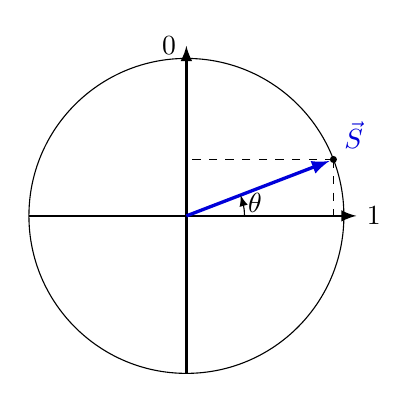
\begin{tikzpicture}[scale=2]
    \tikzset{>=latex}
    \def\xmax{1.0}
    \def\ul{0.6}
    \def\R{1.0}

    \def\ang{21}
    \coordinate (O) at (0,0);
    \coordinate (X) at (\xmax,0);
    \coordinate (R) at (\ang:\R);
    \draw[->,line width=0.9] (-\xmax,0) -- (1.08*\xmax,0) node[right] {$1$};
    \draw[->,line width=0.9] (0,-\xmax) -- (0,1.08*\xmax) node[left] {$0$};
    \node[fill=black,circle,inner sep=0.9] (R') at (R) {};
    \draw[->,very thick,blue!85!black] (O) -- (R') node[above right] {$\vec{S}$};
    \draw pic[->,"$\theta$",draw=black,angle radius=21,angle eccentricity=1.2] {angle=X--O--R};
    \draw (O) circle (\R);
    \draw[dashed] (R) -- ({\R*cos(\ang)},0);
    \draw[dashed] (R) -- (0,{\R*sin(\ang)});
  \end{tikzpicture}
\end{center}
\begin{enumerate}[label=(\alph*)]
  \item How many states are possible for the qubit to be in?
  \item If it is classical bit where would you draw your vector that represents classical state?
  \item If the vector makes an angle 45 degree with the $x$-axis, how would you represent the qubit state mathematically?
  \item If the vector makes an angle of 135 degrees with $x$-axis, how would your response to (c) change?
\end{enumerate}
\end{problem}
\begin{soln}~
  \begin{enumerate}[label=(\alph*)]
    \item There are an infinite number of possible states as the cardinality of $[0,1]$---the set of possible values for the components of the state vector---is the same as the cardinality of $\mathbb{R}$. This can be shown several ways,
          one of which is through the bijection established somewhat informally by the fact that $[0,1]$ clearly injects into $\mathbb{R}$ as $[0,1]\subset\mathbb{R}$
          and $x\mapsto \frac{2\left[\arctan(x)+\frac{\pi}{2}\right]}{\pi}$ which injects $\mathbb{R}$ into $[0,1]$ by virtue of the periodic nature of $\arctan$.
    \item Here the blue vectors represent classical states 0 and 1 and the green vector represents some arbitrary quantum state
          \begin{center}
            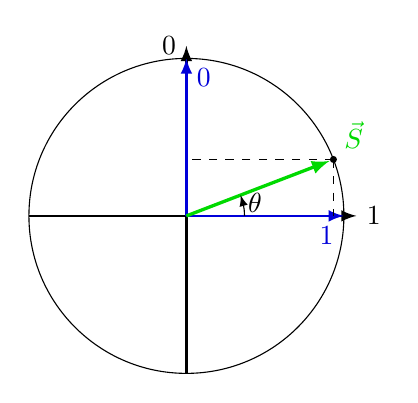
\begin{tikzpicture}[scale=2]
              \tikzset{>=latex}
              \def\xmax{1.0}
              \def\ul{0.6}
              \def\R{1.0}

              \def\ang{21}
              \coordinate (O) at (0,0);
              \coordinate (X) at (\xmax,0);
              \coordinate (R) at (\ang:\R);
              \draw[->,line width=0.9] (-\xmax,0) -- (1.08*\xmax,0) node[right] {$1$};
              \draw[->,line width=0.9] (0,-\xmax) -- (0,1.08*\xmax) node[left] {$0$};
              \draw[->,line width=0.9,blue!85!black] (0,0) -- (\xmax,0) node[below left] {$1$};
              \draw[->,line width=0.9,blue!85!black] (0,0) -- (0,\xmax) node[below right] {$0$};
              \node[fill=black,circle,inner sep=0.9] (R') at (R) {};
              \draw[->,very thick,green!85!black] (O) -- (R') node[above right] {$\vec{S}$};
              \draw pic[->,"$\theta$",draw=black,angle radius=21,angle eccentricity=1.2] {angle=X--O--R};
              \draw (O) circle (\R);
              \draw[dashed] (R) -- ({\R*cos(\ang)},0);
              \draw[dashed] (R) -- (0,{\R*sin(\ang)});
            \end{tikzpicture}
          \end{center}
    \item $\displaystyle\vec{S}=\left(\cos\left(\frac{\pi}{4}\right),\sin\left(\frac{\pi}{4}\right)\right)=\left(\frac{\sqrt{2}}{2},\frac{\sqrt{2}}{2}\right)$
    \item $\displaystyle\vec{S}=\left(\cos\left(\frac{3\pi}{4}\right),\sin\left(\frac{3\pi}{4}\right)\right)=\left(\frac{\sqrt{2}}{2},-\frac{\sqrt{2}}{2}\right)$ 
    which is perfectly fine as we end up squaring the magnitudes of the components when talking about probability.
  \end{enumerate}
\end{soln}

% PROBLEM 3
\begin{problem}~
\begin{enumerate}[label=(\alph*)]
  \item Can a scalar be a complex number?
  \item Given entries i , -i, 1+i create a column vector $A$ and find
        \begin{enumerate}[label=(\roman*)]
          \item $A^\dagger$
          \item $A^\dagger A$
        \end{enumerate}
  \item Which of the following matrices are unitary matrices?
        $$
          \begin{bmatrix}
            1   & 1-i \\
            1+i & 4
          \end{bmatrix}\qquad\qquad\qquad
          \frac{1}{5}\begin{bmatrix}
            -1+2i & -4-2i \\
            2-4i  & -2-i
          \end{bmatrix}
        $$
  \item Can the following matrices be Hermitian? Why?
        $$
          \begin{bmatrix}
            0 & -i \\
            i & 0
          \end{bmatrix}\qquad\qquad\qquad
          \frac{1}{5}\begin{bmatrix}
            1   & 2-i  & 3-i  \\
            2+i & 3    & 1+2i \\
            3+i & 1-2i & 7
          \end{bmatrix}
        $$
\end{enumerate}
\end{problem}
\begin{soln}~
  \begin{enumerate}[label=(\alph*)]
    \item Yes. Just as any element of $\mathbb{Z},\mathbb{Q},\mathbb{R}\ldots$ is a scalar, so is any element of $\mathbb{C}$.
    \item $\displaystyle A=\begin{bmatrix}
              i  \\
              -i \\
              1+i
            \end{bmatrix}$
          \begin{enumerate}[label=(\roman*)]
            \item $A^\dagger=(A^T)^*=\begin{bmatrix}
                      -i & i & 1-i
                    \end{bmatrix}$
            \item $A^\dagger A=\begin{bmatrix}
                      -i & i & 1-i
                    \end{bmatrix}\begin{bmatrix}
                      i  \\
                      -i \\
                      1+i
                    \end{bmatrix}=\begin{bmatrix}
                      1 & 1 & 2
                    \end{bmatrix}$
          \end{enumerate}
    \item Which of the following matrices are unitary matrices?
          $$
            \begin{bmatrix}
              1   & 1-i \\
              1+i & 4
            \end{bmatrix}            \begin{bmatrix}
              1   & 1+i \\
              1-i & 4
            \end{bmatrix}=\begin{bmatrix}
              1-2i & 5-3i  \\
              3+i  & 16+2i
            \end{bmatrix}\neq I_2 \therefore \text{not unitary}
          $$
          $$
            \begin{bmatrix}
              -1+2i & -4-2i \\
              2-4i  & -2-i
            \end{bmatrix}\begin{bmatrix}
              -1-2i & -4+2i \\
              2+4i  & -2+i
            \end{bmatrix}=
            \begin{bmatrix}
              5-20i   & 10-10i \\
              -10-10i & 5+20i
            \end{bmatrix}\neq I_2 \therefore \text{not unitary}
          $$
    \item Both matrices are, by inspection, Hermitian as both are square and have mirrored-conjugate non-diagonal elements which means $A=A^\dagger$.
  \end{enumerate}
\end{soln}

% PROBLEM 4
\begin{problem} Find the eigenvalues and eigenvectors of
\begin{enumerate}[label=(\alph*)]
  \item $$\begin{bmatrix}
            0 & i \\
            1 & 0
          \end{bmatrix}$$
  \item $$\begin{bmatrix}
            0 & i \\
            i & 0
          \end{bmatrix}$$
\end{enumerate}
\end{problem}
\begin{soln}~
  \begin{enumerate}[label=(\alph*)]
    \item Eigenvalues:
          \begin{align*}
            0 =      & \,\det(A-\lambda I) \\
            =        &
            \det(\begin{bmatrix}
                     0 & i \\
                     1 & 0
                   \end{bmatrix}
            -
            \begin{bmatrix}
                \lambda & 0       \\
                0       & \lambda
              \end{bmatrix})
            =
            \begin{vmatrix}
              -\lambda & i        \\
              1        & -\lambda
            \end{vmatrix}            \\
            =        & \lambda^2-i         \\
            \implies & \lambda=\pm\sqrt{i}
          \end{align*}
          Eigenvectors:
          \begin{align*}
            \begin{bmatrix}
              -\sqrt{i} & i         & 0 \\
              1         & -\sqrt{i} & 0
            \end{bmatrix}\sim
            \begin{bmatrix}
              -1 & \sqrt{i}  & 0 \\
              1  & -\sqrt{i} & 0
            \end{bmatrix}\sim
            \begin{bmatrix}
              -1 & \sqrt{i} & 0 \\
              0  & 0        & 0
            \end{bmatrix}
            \implies & \vec{v}_1=\begin{bmatrix}
                                   \sqrt{i} \\
                                   1
                                 \end{bmatrix} \\
            \begin{bmatrix}
              \sqrt{i} & i        & 0 \\
              1        & \sqrt{i} & 0
            \end{bmatrix}\sim
            \begin{bmatrix}
              1 & \sqrt{i}  & 0 \\
              1 & -\sqrt{i} & 0
            \end{bmatrix}\sim
            \begin{bmatrix}
              1 & \sqrt{i} & 0 \\
              0 & 0        & 0
            \end{bmatrix}
            \implies & \vec{v}_2=\begin{bmatrix}
                                   -\sqrt{i} \\
                                   1
                                 \end{bmatrix}
          \end{align*}

    \item Eigenvalues:
          \begin{align*}
            0 =      & \det(\begin{bmatrix}
                              0 & i \\
                              i & 0
                            \end{bmatrix}
            -
            \begin{bmatrix}
              \lambda & 0       \\
              0       & \lambda
            \end{bmatrix})
            =
            \begin{vmatrix}
              -\lambda & i        \\
              i        & -\lambda
            \end{vmatrix}            \\
            =        & \lambda^2+1         \\
            \implies & \lambda=\pm i
          \end{align*}
          Eigenvectors
          \begin{align*}
            \begin{bmatrix}
              -i & i  & 0 \\
              i  & -i & 0
            \end{bmatrix}\sim
            \begin{bmatrix}
              -1 & 1  & 0 \\
              1  & -1 & 0
            \end{bmatrix}\sim
            \begin{bmatrix}
              -1 & 1 & 0 \\
              0  & 0 & 0
            \end{bmatrix}
            \implies & \vec{v}_1=\begin{bmatrix}
                                   1 \\
                                   1
                                 \end{bmatrix} \\
            \begin{bmatrix}
              i & i & 0 \\
              i & i & 0
            \end{bmatrix}\sim
            \begin{bmatrix}
              1 & 1 & 0 \\
              1 & 1 & 0
            \end{bmatrix}\sim
            \begin{bmatrix}
              1 & 1 & 0 \\
              0 & 0 & 0
            \end{bmatrix}
            \implies & \vec{v}_2=\begin{bmatrix}
                                   -1 \\
                                   1
                                 \end{bmatrix}
          \end{align*}
  \end{enumerate}
\end{soln}
\end{document}